\chapter{Experiments}
\label{ch:experiments}

\section{Datasets}
\label{sec:ds}

In this section we consider datasets that are separated in two opposing communities. The information about the opinions of each member of this community is known. Thus, we can assign internal opinions -1 and 1 to the nodes depending on their community membership\cite{tsapMatakosTerzi}.  We consider the following.

\begin{enumerate}

  \item The Karate dataset, that represents the friendships between the members of a karate club at a US university. This network is split in two equal size polarized communities around two rival karate instructors.
  
  \item The Books dataset, that is a network of US politics books. These books were published near the 2004 presidential election and sold by Amazon. These Books are classified as "Liberal", "Conservative", or "Neutral".  There are in total 43 liberal books, 49 conservative and 13 neutral.
  
  \item The Blogs dataset, a network of hyperlinks between online blogs on US politics. Blogs are classified as either Liberal or Conservative.
  
  \item The Elections dataset, this dataset is the network between the Twitter followers of Hillary Clinton and Donald Trump collected in the period 15/12/2016-15/01/2017 – around the time of the 2016 presidential elections. Members of this network are assigned an internal opinion of 1 or -1 based on which one of the two candidates they follow. We took a subsampled portion that has be done by Matakos, et al \cite{tsapMatakosTerzi}.
    
  \item The beefban dataset, a  hashtag that Twitter users used in March 2015 to signal that their posts referred to a decision by the Indian government about the consumption of beef meat in India.
  
  \item The GermanWings dataset, a  hashtag that Twitter users used after the crash of GermanWings Flight 9525.
  
\end{enumerate}


\section{Dataset statistics}
\label{sec:stats}

\begin{table}[H]
 \centering
 \caption{Stats}
 \label{tab:statistics}
 \begin{tabular}{| l || l | l | l | l |}
 \hline
  Name & \# of Nodes & \# of Edges & Avg. Degree & $\pi(z)$\\
  \hline
  \hline
  Karate & $34$ & $78$ & 4.5882 &  0.33964\\
  \hline
    books & $105$ & $441$ & 8.4 &  0.43429\\
  \hline
    beefban & $799$ & $6026$ & 15.0839 &  0.30326\\
  \hline
  polblogs & $1490$ & $16718$ & 22.4403 &  0.30983\\
  \hline
  GermanWings & $2111$ & $7329$ & 6.9436 &  0.44479\\
  \hline
  ClintonTrump & $2832$ & $18551$ & 13.1010 &  0.07582\\
  \hline
 \end{tabular}
 \end{table}
 
\vspace{20pt}
\clearpage

\section{A Visualisation of Edge Additions}
\label{sec:vis}

\begin{figure}[!htbp]
	\centering
	\captionsetup{justification=centering,margin=2cm}
	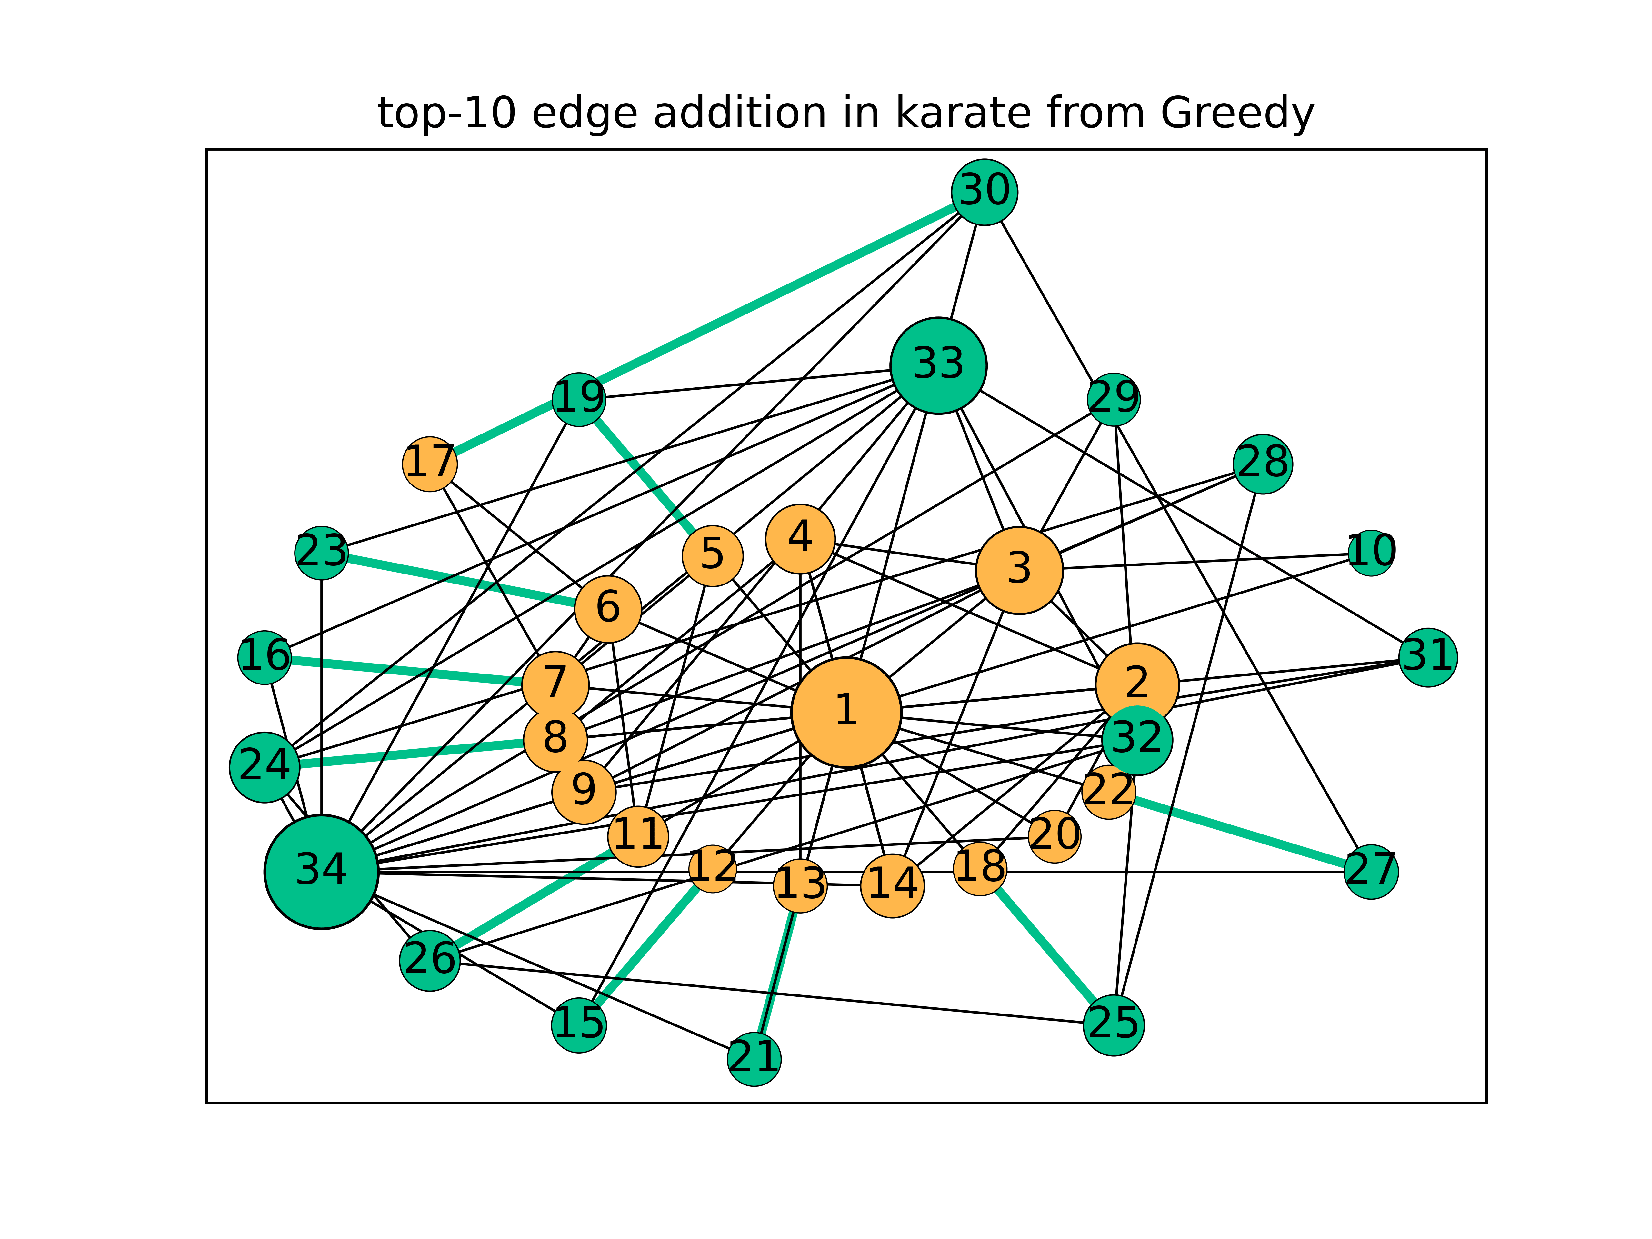
\includegraphics[width=0.65\textwidth]{Figures/top-10_karate_greedy}
	\caption{the top-10 edges proposed by the greedy algorithm}
	\label{fig:top-10-karate}
\end{figure}

\section{Results}
\label{sec:experim}

All experiments were made with an 2,7 GHz Dual-Core Intel Core i5 on the PyCharm IDE. We can only experiment with the $Karate$ and the $Books$ dataset on all the heuristics. The $Greedy$ algorithm cannot run on the rest of the datasets because they contain thousands of nodes. The $Greedy$ algorithm needs to consider changes in the network structure so it is impossible to compute the polarization so many times.
\\
\\ 
The same applies for the $GreedyBatch$ algorithm. Although the $GreedyBatch$ algorithm can run on the $beefban$ dataset that contains $799$ nodes it would take a lot of time even for the $polblogs$ dataset that has $1490$ nodes.
\\
\\
The $FirstTopGreedy$ and the $Expressed Opinion$ can run in all datasets but provide us with a small decrease in polarization. This decrease can be greater if we consider edge additions that are proportional to the size of the dataset. Greater number of edges would make $FirstTopGreedy$ nonrunnable. The $Expressed Opinion$ can run in our larger datasets even with a big number of additions.
\clearpage


\subsection{Experiments with Heuristics}


\begin{figure}[!htbp]
	\centering
	\captionsetup{justification=centering,margin=2cm}
	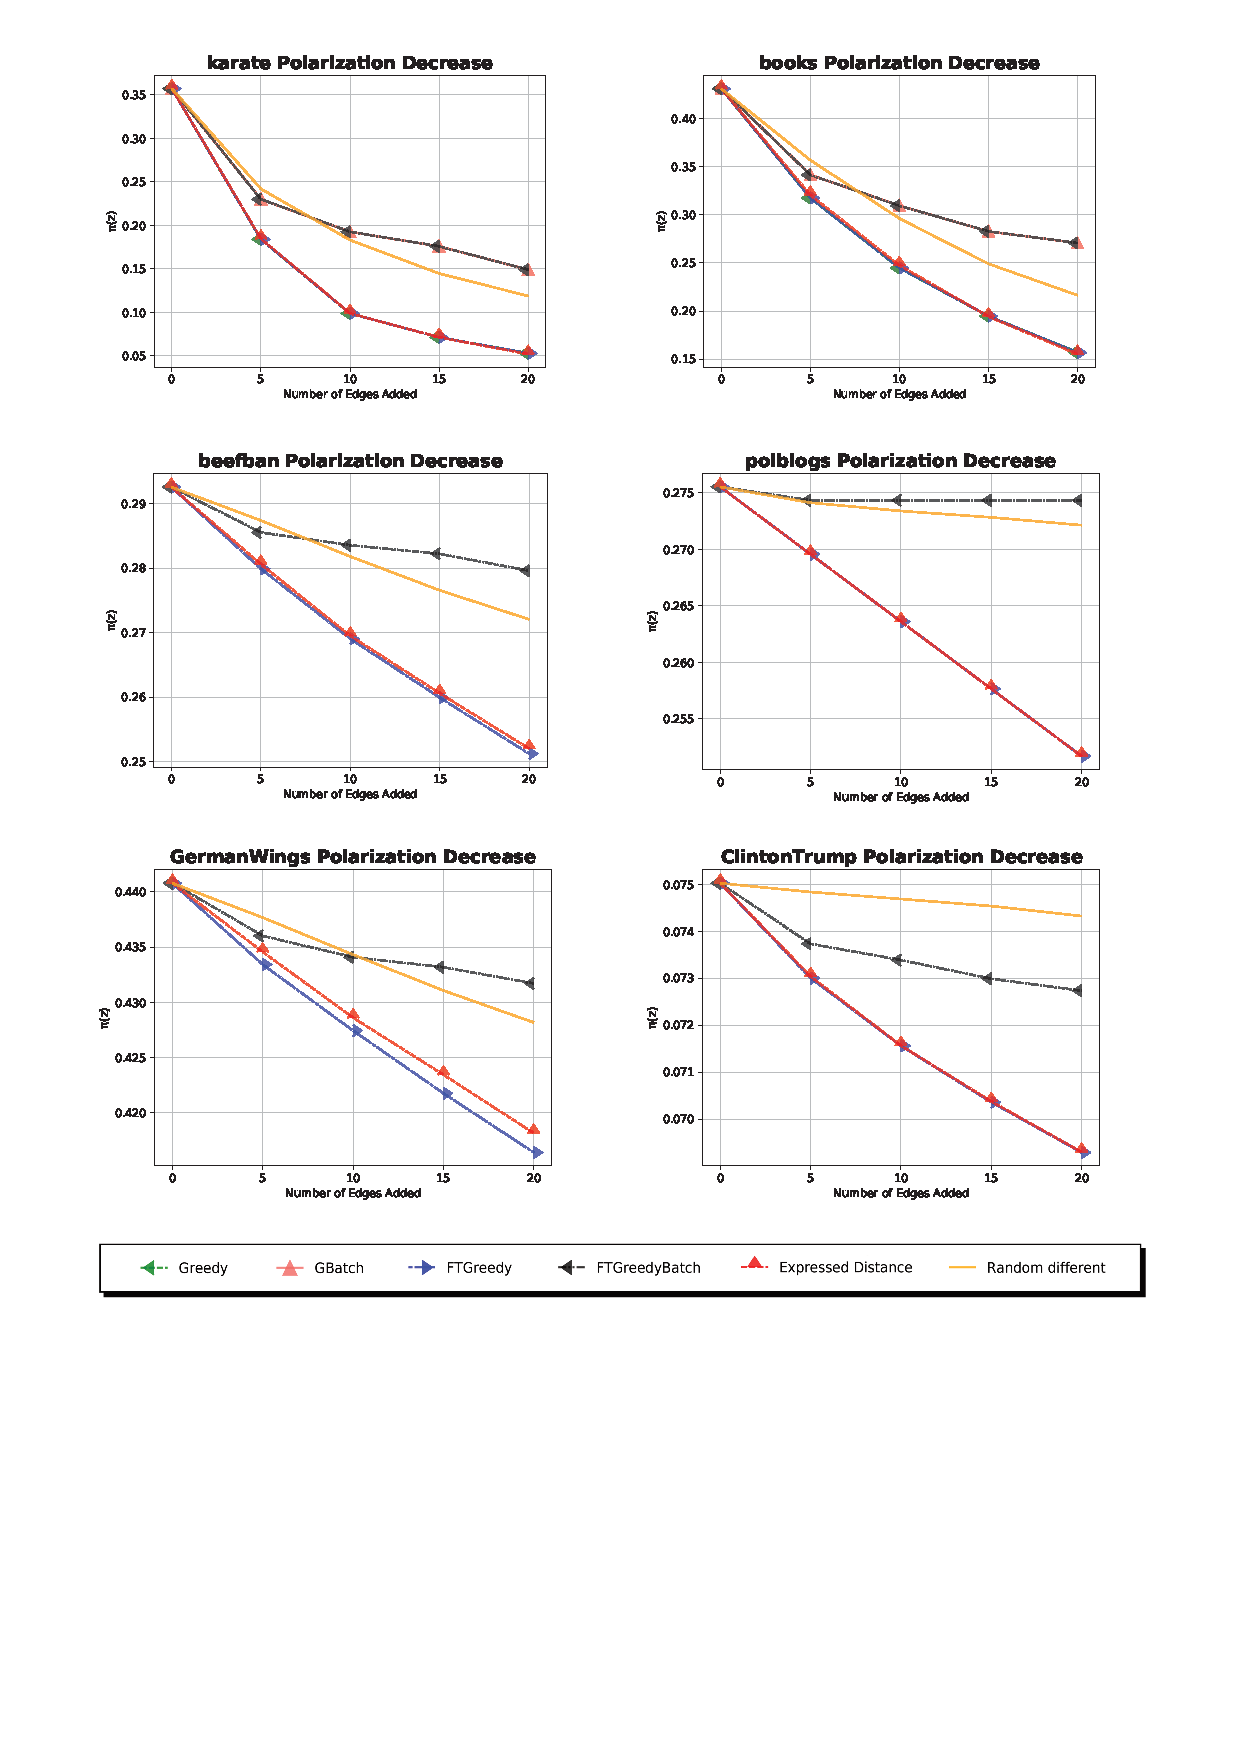
\includegraphics[width=0.90\textwidth]{Figures/heuristics_small}
	\caption{Comparison of the heuristics between datasets}
	\label{fig:heuristics_small}
\end{figure}

\noindent We start by applying the heuristics described at~\ref{sec:heuristics} in these 6 datasets. The algorithms perform as expected. The greedy ones have better results but are expensive in time. The $Greedy Batch$ algorithms perform slightly worse but need less time to run. 
\\
Finally the $Distance/Multiplication$ algorithms are cheap on time but do not perform well. 
In almost all cases they are worse than the $Random$ addition algorithm.
This is due to the fact that they do not take into consideration the structural  changes of the graph after an addition. 
\\
\\
Their choice is based on the vector of expressed opinions. This vector after some additions will be completely different from what the algorithm knew and thus will make decisions with a false view. The price we pay to recompute this vector is the same as the greedy one.
\clearpage

\begin{figure}[!htbp]
	\centering
	\captionsetup{justification=centering,margin=2cm}
	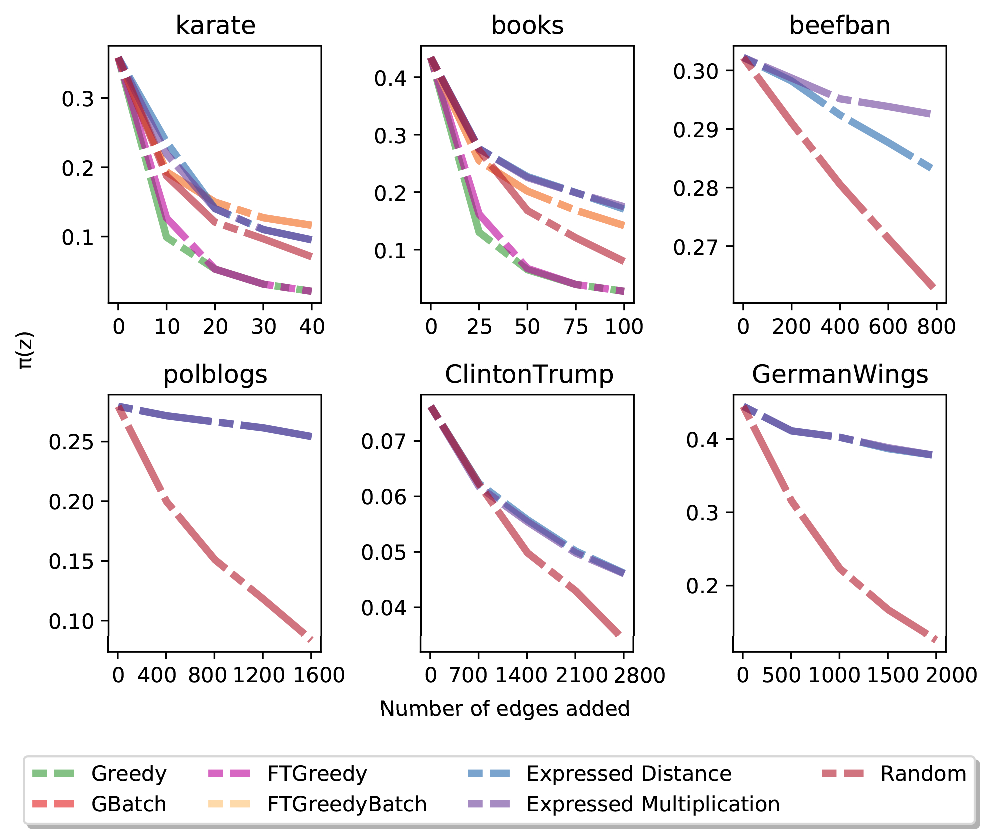
\includegraphics[width=0.90\textwidth]{Figures/heuristics_big}
	\caption{Comparison of the heuristics between datasets}
	\label{fig:heuristics_bigl}
\end{figure}

\vspace{20pt}

\noindent This behaviour can be seen more clear when we attempt to add edges proportional to the size of the graph. 
\\
\\
The random addition will almost drop to zero and the $Distance/Multiplication$ algorithm will still struggle to have a decent decrease. The $Greedy$ ones still perform as expected.
\\
\\ 
We can not run the $Greedy$ algorithms in larger datasets due to time limitations.
\clearpage


\subsection{Experiments by including probabilities}
\label{probexperiment}

\begin{figure}[!htbp]
	\centering
	\captionsetup{justification=centering,margin=2cm}
	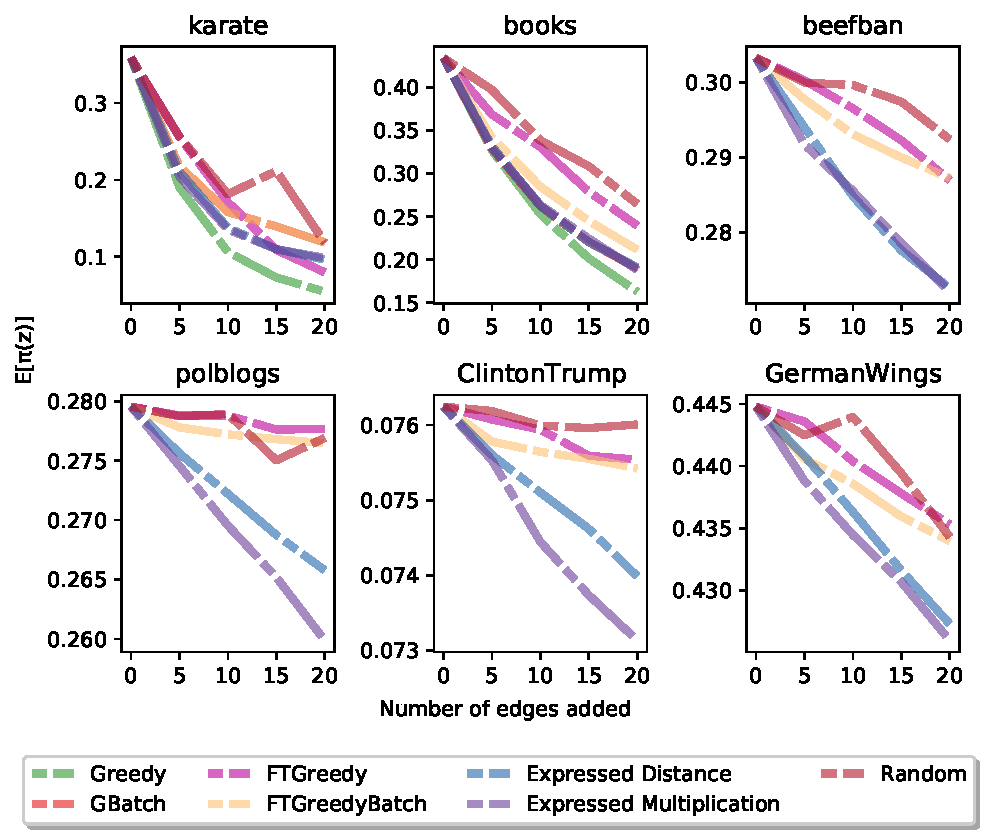
\includegraphics[width=0.90\textwidth]{Figures/embeddings_small}
	\caption{Comparison of the Expected Decrease between datasets}
	\label{fig:embeddings_smalll}
\end{figure}


\clearpage
